\subsection{Eigenvalues distribution}
\label{sec:dist}

One way to investigate if there is any significant difference between the regular and random SOMs is to compare their neural responses to the same random stimuli. Therefore, we measure the neural activity and build a covariance matrix out of it. Then, we compute the eigenvalues of the covariance matrix (or Gram matrix) and we estimate a probability distribution. Thus, we can compare the eigenvalues distributions of the two maps and compare them to each other. If the distributions are close enough in the sense of Wasserstein distance then the two SOMs are similar in terms of neural activation.  A Gram matrix is an $n \times n$ matrix given by where $n$ is the number of neurons of the map and ${\bf Y} \in \mathbb{R}^{n \times m}$ is a matrix for which each column is the activation of all $n$ neurons to a random stimulus.

From a computational point of view we construct the matrix ${\bf Y}$ by applying a set of stimuli to the self-organized map and computing the activity of each neuron within the map. This implies that ${\bf Y} \in \mathbb{R}^{m \times n}$, where $m=1024$ (the number of neurons) and $n={2, 3}$ (two- or three-dimensional input samples). Then we compute the covariance or Gram matrix as ${\bf M} = {\bf Y}{\bf Y}^T \in \mathbb{R}^{n \times n}$, where $n$ is the number of neurons. Then we compute the eigenvalues and obtain their distribution by sampling the activity of neurons of each experiment for $200$ different initial conditions using $50$ input sample each time. At the end of sampling we get an \emph{ensemble} of $200$ Gram matrices and finally we estimate the probability density of the eigenvalues on each \emph{ensemble} by applying a Kernel Density Estimation method~\citep{Parzen:1962} (KDE) with a Gaussian kernel and bandwidth $h=0.4$. This allows us to quantify any differences on the distributions of the regular and randomized SOMs by calculating the Earth-Mover or Wasserstein-1 distance over the two distributions (regular ($P$) and random SOM ($Q$)). The Wasserstein distance is computed as $W(P, Q) = \inf_{\gamma \in \Pi(P, Q)}\{\mathbb{E}_{(x, y) \sim \gamma}\Big[||x - y||\Big]\}$, where $\Pi(P, Q)$ denotes the set of all joint distributions $\gamma (x, y)$, whose marginals are $P$ and $Q$, respectively. Intuitively, $\gamma (x,y)$ indicates  how  much ``mass'' must be transported from $x$ to $y$ to transform the distribution $P$ into the distribution $Q$. 

The distributions of the eigenvalues of the RSOM and the regular SOM are shown on figure~\ref{fig:eigenvalues}. We can conclude that the two distributions are alike and do not suggest any significant difference between the two maps in terms of neural activity. This implies that the RSOM and the regular SOM have similar statistics of their neural activities. This means that the loss of information and the \emph{stretch} to the input data from both RSOM and regular SOM are pretty close and the underlying  topology of the two maps do not really affect the neural activity. This is also confirmed
by measuring the Wasserstein distance between the two distributions. The blue curve shows the regular SOM or distribution $P$ and the black curve the RSOM or distribution $Q$. The Wasserstein distance between the two distributions $P$ and $Q$ indicates that the two distributions are nearly identical on all datasets. The Wasserstein distances in Table~\ref{table:distances}
confirm that the eigenvalues distributions of SOM and RSOM are almost identical indicating that both maps retain the
same amount of information after learning the representations of input spaces.

\begin{table}[!ht]
  \begin{center}
    \begin{tabular}{ll}
        \textbf{Experiment} & \textbf{Wasserstein Distance} \\
        \hline
        $2$D ring dataset               & $0.0000323$\\
        $2$D uniform dataset with holes & $0.0000207$  \\
        $3$D uniform dataset            & $0.0001583$ \\
        MNIST dataset                   & $0.0015$ \\
    \end{tabular}
      \caption{\textbf{Wasserstein distances of eigenvalues distributions.} We report here the Wasserstein 
      distances between eigenvalues distributions of SOM and RSOM for each of the four major experiments we
      ran. The results indicate that the distributions are close pointing out that the SOM and RSOM capture
      a similar level of information during training. For more information regarding how we computed the 
      eigenvalues distributions and the Wasserstein distance please see Section~\ref{sec:dist}.}
      \label{table:distances}
  \end{center}
\end{table}

\begin{figure}
  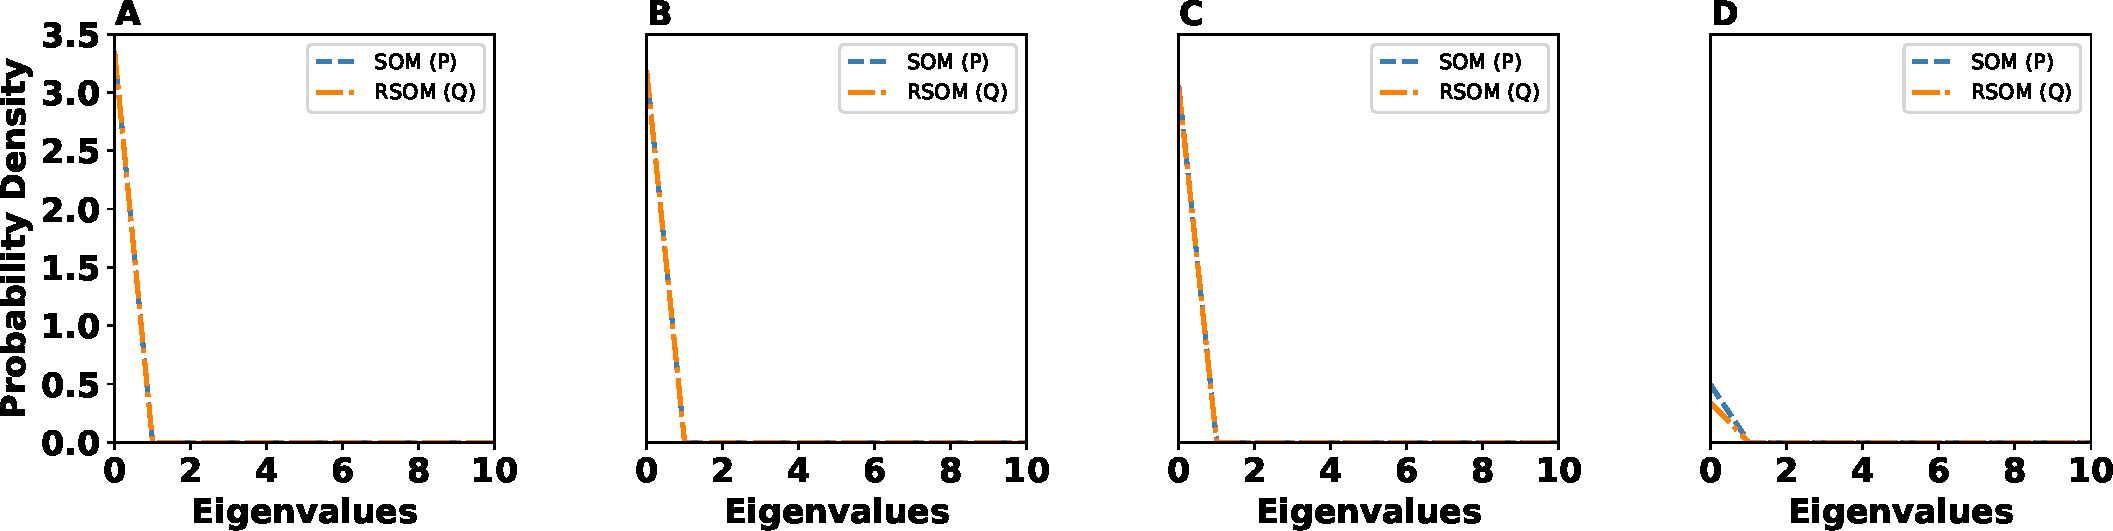
\includegraphics[width=\columnwidth]{eig-distributions-new.pdf}
  %
  \caption{Eigenvalues distribution for \textbf{A} 2D Ring dataset \textbf{B} 2D uniform dataset with holes \textbf{C} 3D uniform dataset and \textbf{D} MNIST Dataset
  }%
  \label{fig:eigenvalues}
 \end{figure}